\documentclass[twoside]{book}

% Packages required by doxygen
\usepackage{fixltx2e}
\usepackage{calc}
\usepackage{doxygen}
\usepackage[export]{adjustbox} % also loads graphicx
\usepackage{graphicx}
\usepackage[utf8]{inputenc}
\usepackage{makeidx}
\usepackage{multicol}
\usepackage{multirow}
\PassOptionsToPackage{warn}{textcomp}
\usepackage{textcomp}
\usepackage[nointegrals]{wasysym}
\usepackage[table]{xcolor}

% Font selection
\usepackage[T1]{fontenc}
\usepackage[scaled=.90]{helvet}
\usepackage{courier}
\usepackage{amssymb}
\usepackage{sectsty}
\renewcommand{\familydefault}{\sfdefault}
\allsectionsfont{%
  \fontseries{bc}\selectfont%
  \color{darkgray}%
}
\renewcommand{\DoxyLabelFont}{%
  \fontseries{bc}\selectfont%
  \color{darkgray}%
}
\newcommand{\+}{\discretionary{\mbox{\scriptsize$\hookleftarrow$}}{}{}}

% Page & text layout
\usepackage{geometry}
\geometry{%
  a4paper,%
  top=2.5cm,%
  bottom=2.5cm,%
  left=2.5cm,%
  right=2.5cm%
}
\tolerance=750
\hfuzz=15pt
\hbadness=750
\setlength{\emergencystretch}{15pt}
\setlength{\parindent}{0cm}
\setlength{\parskip}{3ex plus 2ex minus 2ex}
\makeatletter
\renewcommand{\paragraph}{%
  \@startsection{paragraph}{4}{0ex}{-1.0ex}{1.0ex}{%
    \normalfont\normalsize\bfseries\SS@parafont%
  }%
}
\renewcommand{\subparagraph}{%
  \@startsection{subparagraph}{5}{0ex}{-1.0ex}{1.0ex}{%
    \normalfont\normalsize\bfseries\SS@subparafont%
  }%
}
\makeatother

% Headers & footers
\usepackage{fancyhdr}
\pagestyle{fancyplain}
\fancyhead[LE]{\fancyplain{}{\bfseries\thepage}}
\fancyhead[CE]{\fancyplain{}{}}
\fancyhead[RE]{\fancyplain{}{\bfseries\leftmark}}
\fancyhead[LO]{\fancyplain{}{\bfseries\rightmark}}
\fancyhead[CO]{\fancyplain{}{}}
\fancyhead[RO]{\fancyplain{}{\bfseries\thepage}}
\fancyfoot[LE]{\fancyplain{}{}}
\fancyfoot[CE]{\fancyplain{}{}}
\fancyfoot[RE]{\fancyplain{}{\bfseries\scriptsize Generated by Doxygen }}
\fancyfoot[LO]{\fancyplain{}{\bfseries\scriptsize Generated by Doxygen }}
\fancyfoot[CO]{\fancyplain{}{}}
\fancyfoot[RO]{\fancyplain{}{}}
\renewcommand{\footrulewidth}{0.4pt}
\renewcommand{\chaptermark}[1]{%
  \markboth{#1}{}%
}
\renewcommand{\sectionmark}[1]{%
  \markright{\thesection\ #1}%
}

% Indices & bibliography
\usepackage{natbib}
\usepackage[titles]{tocloft}
\setcounter{tocdepth}{3}
\setcounter{secnumdepth}{5}
\makeindex

% Hyperlinks (required, but should be loaded last)
\usepackage{ifpdf}
\ifpdf
  \usepackage[pdftex,pagebackref=true]{hyperref}
\else
  \usepackage[ps2pdf,pagebackref=true]{hyperref}
\fi
\hypersetup{%
  colorlinks=true,%
  linkcolor=blue,%
  citecolor=blue,%
  unicode%
}

% Custom commands
\newcommand{\clearemptydoublepage}{%
  \newpage{\pagestyle{empty}\cleardoublepage}%
}

\usepackage{caption}
\captionsetup{labelsep=space,justification=centering,font={bf},singlelinecheck=off,skip=4pt,position=top}

%===== C O N T E N T S =====

\begin{document}

% Titlepage & ToC
\hypersetup{pageanchor=false,
             bookmarksnumbered=true,
             pdfencoding=unicode
            }
\pagenumbering{roman}
\begin{titlepage}
\vspace*{7cm}
\begin{center}%
{\Large My Project }\\
\vspace*{1cm}
{\large Generated by Doxygen 1.8.11}\\
\end{center}
\end{titlepage}
\clearemptydoublepage
\tableofcontents
\clearemptydoublepage
\pagenumbering{arabic}
\hypersetup{pageanchor=true}

%--- Begin generated contents ---
\chapter{File Index}
\section{File List}
Here is a list of all documented files with brief descriptions\+:\begin{DoxyCompactList}
\item\contentsline{section}{\hyperlink{ARN_8cpp}{A\+R\+N.\+cpp} }{\pageref{ARN_8cpp}}{}
\item\contentsline{section}{{\bfseries A\+R\+N.\+h} }{\pageref{ARN_8h}}{}
\end{DoxyCompactList}

\chapter{File Documentation}
\hypertarget{ARN_8cpp}{}\section{A\+R\+N.\+cpp File Reference}
\label{ARN_8cpp}\index{A\+R\+N.\+cpp@{A\+R\+N.\+cpp}}
{\ttfamily \#include \char`\"{}A\+R\+N.\+h\char`\"{}}\\*
{\ttfamily \#include $<$iostream$>$}\\*
{\ttfamily \#include $<$string$>$}\\*
Include dependency graph for A\+R\+N.\+cpp\+:\nopagebreak
\begin{figure}[H]
\begin{center}
\leavevmode
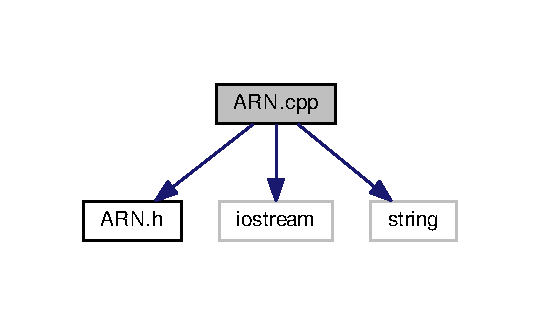
\includegraphics[width=259pt]{ARN_8cpp__incl}
\end{center}
\end{figure}
\subsection*{Functions}
\begin{DoxyCompactItemize}
\item 
int {\bfseries main} (int argc, char $\ast$argv\mbox{[}$\,$\mbox{]})\hypertarget{ARN_8cpp_a0ddf1224851353fc92bfbff6f499fa97}{}\label{ARN_8cpp_a0ddf1224851353fc92bfbff6f499fa97}

\item 
char $\ast$ \hyperlink{ARN_8cpp_ac39e6a29f85f490e595b4934bf045e4e}{traducir\+A\+R\+Na\+AA} (char $\ast$orig, int size)
\item 
void \hyperlink{ARN_8cpp_abe553055efef51b7180cf3761659682b}{imprimir\+Arreglo\+De\+Char} (char $\ast$str, int num)
\item 
bool \hyperlink{ARN_8cpp_aeea50fcfde521778d1a7549e664ce888}{checkeo\+Argumentos} (int argc, char $\ast$argv\mbox{[}$\,$\mbox{]})
\item 
char \hyperlink{ARN_8cpp_af8b80c835550e9ea910d5d8144ddbf7a}{next\+Seq} (char $\ast$sub)
\end{DoxyCompactItemize}


\subsection{Detailed Description}
Programa que traduce una cadena de A\+RN en la correspondiente cadena de aminoácidos. 

\subsection{Function Documentation}
\index{A\+R\+N.\+cpp@{A\+R\+N.\+cpp}!checkeo\+Argumentos@{checkeo\+Argumentos}}
\index{checkeo\+Argumentos@{checkeo\+Argumentos}!A\+R\+N.\+cpp@{A\+R\+N.\+cpp}}
\subsubsection[{\texorpdfstring{checkeo\+Argumentos(int argc, char $\ast$argv[])}{checkeoArgumentos(int argc, char *argv[])}}]{\setlength{\rightskip}{0pt plus 5cm}bool checkeo\+Argumentos (
\begin{DoxyParamCaption}
\item[{int}]{argc, }
\item[{char $\ast$}]{argv\mbox{[}$\,$\mbox{]}}
\end{DoxyParamCaption}
)}\hypertarget{ARN_8cpp_aeea50fcfde521778d1a7549e664ce888}{}\label{ARN_8cpp_aeea50fcfde521778d1a7549e664ce888}
Revisa los argumentos que recibe el programa. 
\begin{DoxyParams}{Parameters}
{\em argc} & Cantidad de argumentos. \\
\hline
{\em argv} & Argumentos. \\
\hline
\end{DoxyParams}
\begin{DoxyReturn}{Returns}
Si los argumentos son válidos retorna verdadero. 
\end{DoxyReturn}
\index{A\+R\+N.\+cpp@{A\+R\+N.\+cpp}!imprimir\+Arreglo\+De\+Char@{imprimir\+Arreglo\+De\+Char}}
\index{imprimir\+Arreglo\+De\+Char@{imprimir\+Arreglo\+De\+Char}!A\+R\+N.\+cpp@{A\+R\+N.\+cpp}}
\subsubsection[{\texorpdfstring{imprimir\+Arreglo\+De\+Char(char $\ast$str, int num)}{imprimirArregloDeChar(char *str, int num)}}]{\setlength{\rightskip}{0pt plus 5cm}void imprimir\+Arreglo\+De\+Char (
\begin{DoxyParamCaption}
\item[{char $\ast$}]{str, }
\item[{int}]{num}
\end{DoxyParamCaption}
)}\hypertarget{ARN_8cpp_abe553055efef51b7180cf3761659682b}{}\label{ARN_8cpp_abe553055efef51b7180cf3761659682b}
Esta función se encarga de imprimir cierto número de caracteres de un string. 
\begin{DoxyParams}{Parameters}
{\em str} & Puntero a la cadena de caracteres. \\
\hline
{\em num} & Número de caracteres a imprimir. \\
\hline
\end{DoxyParams}
\index{A\+R\+N.\+cpp@{A\+R\+N.\+cpp}!next\+Seq@{next\+Seq}}
\index{next\+Seq@{next\+Seq}!A\+R\+N.\+cpp@{A\+R\+N.\+cpp}}
\subsubsection[{\texorpdfstring{next\+Seq(char $\ast$sub)}{nextSeq(char *sub)}}]{\setlength{\rightskip}{0pt plus 5cm}char next\+Seq (
\begin{DoxyParamCaption}
\item[{char $\ast$}]{sub}
\end{DoxyParamCaption}
)}\hypertarget{ARN_8cpp_af8b80c835550e9ea910d5d8144ddbf7a}{}\label{ARN_8cpp_af8b80c835550e9ea910d5d8144ddbf7a}
Recibe un grupo de 3 caracteres correspondientes a un codón y los traduce a un áminoacido. 
\begin{DoxyParams}{Parameters}
{\em sub} & Puntero al primer caracter. \\
\hline
\end{DoxyParams}
\begin{DoxyReturn}{Returns}
Caracter que representa al aminoácido traducido. 
\end{DoxyReturn}
\index{A\+R\+N.\+cpp@{A\+R\+N.\+cpp}!traducir\+A\+R\+Na\+AA@{traducir\+A\+R\+Na\+AA}}
\index{traducir\+A\+R\+Na\+AA@{traducir\+A\+R\+Na\+AA}!A\+R\+N.\+cpp@{A\+R\+N.\+cpp}}
\subsubsection[{\texorpdfstring{traducir\+A\+R\+Na\+A\+A(char $\ast$orig, int size)}{traducirARNaAA(char *orig, int size)}}]{\setlength{\rightskip}{0pt plus 5cm}char$\ast$ traducir\+A\+R\+Na\+AA (
\begin{DoxyParamCaption}
\item[{char $\ast$}]{orig, }
\item[{int}]{size}
\end{DoxyParamCaption}
)}\hypertarget{ARN_8cpp_ac39e6a29f85f490e595b4934bf045e4e}{}\label{ARN_8cpp_ac39e6a29f85f490e595b4934bf045e4e}
Retorna un arreglo de caracteres con la traduccion a aminoacidos de una cadena de A\+RN. Reserva la memoria necesaria automáticamente, el usuario es responsable de liberarla. 
\begin{DoxyParams}{Parameters}
{\em orig} & Arreglo de caracteres que representa la cadena de A\+RN. \\
\hline
{\em size} & Tamaño de orig. \\
\hline
\end{DoxyParams}
\begin{DoxyReturn}{Returns}
La cadena de aminoacidos, la funcion reserva el nuevo espacio de memoria. 
\end{DoxyReturn}

%--- End generated contents ---

% Index
\backmatter
\newpage
\phantomsection
\clearemptydoublepage
\addcontentsline{toc}{chapter}{Index}
\printindex

\end{document}
